\Chapter{Egy étterem, több futár, több kiszállítás esete}

\Section{A probléma megfoglmazása}

Jelen eset reprezentálja az egy lerakatos több ügynökös utazó ügynök problémát. Feltételek meghatározásánál nélkülözhetetlen szempont, hogy határokat szabjunk az egyes futároknak, hogy ki milyen területre szállít ki. Ennek meghatározásánál fontos a kiszállítási címek közti táv figyelembe vétele. Ezek meghatározása után maga a probléma leegyszerűsíthető egy klasszikus utazó ügynök problémára.

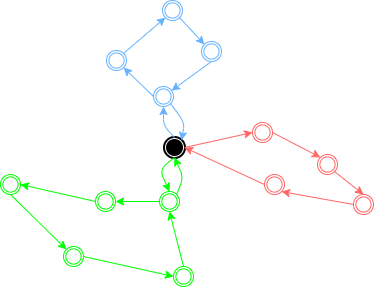
\includegraphics[scale=0.7]{images/Onedepotmtsp.png}

\Section{A probléma megoldása}

\Section{A megoldás implementálása}

\Section{A megoldás tesztelése}
